\documentclass{article}
\usepackage[utf8]{inputenc}
\usepackage{amssymb}
\usepackage{amsfonts}
\usepackage{amsmath}
\usepackage[utf8]{inputenc}
\usepackage[norsk]{babel}
\usepackage{lmodern}
\usepackage{float}
\usepackage{graphicx}
\DeclareGraphicsExtensions{.pdf,.png,.jpg}
\usepackage{latexsym}
\usepackage{hyperref}
\usepackage[euler]{textgreek}
\usepackage{stackengine}
\usepackage{listings}
\usepackage[version-1-compatibility]{siunitx}
\usepackage{pdfpages}
\usepackage{fixltx2e}
\hypersetup{pdfborder={0 0 0}}
\usepackage{pgfplots}
\pgfplotsset{compat=newest}
\pgfplotsset{plot coordinates/math parser=false}
\newlength\figureheight
\newlength\figurewidth
\usepackage[section]{placeins}%Sørger for at plots og andre floats holder seg til sin section.
\setlength\parindent{0pt}%Setter indent til 0



\title{Exercise 3 - TTK4130 Modeling and Simulation}
\author{Camilla Sterud}
\date{}

\begin{document}

\maketitle

\newpage

\section{Problem 1}

\begin{align}
	k_1 &= f(y_n,t_n)\label{eq:k1}\\
	k_2 &= f(y_n + ha_{21}k_1,t_n + hc_2)\label{eq:k2}\\
	y_{n+1} &= y_n + h(b_1k_1 + b_2k_2)\label{eq:ynext}
\end{align}

Taylor expansion of a funciton of two variables:

\begin{equation}\label{eq:taylorexp}
	f(y + \Delta, t + \delta) = f(y,t) + \Delta\frac{\partial f(y,t)}{\partial y} + \delta\frac{\partial f(y,t)}{\partial t} + O(\Delta^2) + O(\delta\Delta) + O(\delta^2)
\end{equation}


\subsection{a}



\begin{equation*}
	\frac{df(y_n,t_n)}{dt}) = \frac{\partial f(y_n,t_n)}{\partial y}\frac{dy}{dt} + \frac{\partial f(y_n,t_n)}{\partial t} = \frac{\partial f(y_n,t_n)}{\partial y}f(y_n,t_n)+ \frac{\partial f(y_n,t_n)}{\partial t}.
\end{equation*}

$a_{21} = c_1 = C$. Taylor expansion of Equation \ref{eq:k2} using Equation \ref{eq:taylorexp}:

\begin{align*}
	k_2 &= f(y_n,t_n) + ha_{21}k_1\frac{\partial f(y,t)}{\partial y} + hc_2\frac{\partial f(y,t)}{\partial t} + O((ha_{21}k_1)^2) + O(h^2c_2a_{21}k_1) + O(h^2c_2^2)\\
	&= k_1 + hC(k_1\frac{\partial f(y,t)}{\partial y} + \frac{\partial f(y,t)}{\partial t}) + O(h^2C^2)
\end{align*}

\begin{equation}\label{eq:k2exp}
	\underline{\underline{k_2 = f(y_n,t_n) + hC\frac{df(y_n,t_n)}{dt} + O(h^2)}}
\end{equation}

\subsection{b}

From p. 518, Egeland \& Gravdal:
A method is of order $p$ if $p$ is the smallest number that satifies

\begin{equation}\label{eq:order}
	y_{n+1} = y_n + hf(y_n,t_n) + ... + \frac{h^p}{p!} \frac{d^{p-1}f(y_n,t_n)}{dt^{p-1}} + O(h^{p+1}).
\end{equation}

Putting the taylor expansion of $k_2$ from Equation \ref{eq:k2exp} and Equation \ref{eq:k1} into Equation \ref{eq:ynext} yields

\begin{align*}
	y_{n+1} &= y_n + hb_1f(y_n,t_n) + hb_2(f(y_n,t_n) + hC\frac{df(y_n,t_n)}{dt} + O(h^2))\\
	y_{n+1} &= y_n + h(b_1+b_2)f(y_n,t_n) + h^2b_2C\frac{df(y_n,t_n)}{dt} + O(h^3) \\
	\Rightarrow b_1+b_2 &= 1 \quad b_2C = \frac{1}{2!}
\end{align*}

\begin{equation*}
	\underline{\underline{c_2 = a_{12} = \frac{1}{2b_2}, \quad b_1 = 1-b_2}}
\end{equation*}


\section{Problem 2}

\begin{lstlisting}[language=Matlab, frame = single, caption = The explicit Euler method implemented i MATLAB,, label=code2a]
hold on; grid on;

kappa = 1.4;
g = 9.81;

h = 0.01;
t = 0:h:10;

y = zeros (2,length(t));
y(1,1) = 2;
y(2,1) = 0;

f = @(Y) [Y(2);g*(Y(1)^(-kappa) - 1)];

for i = 1:(length(t) - 1)
    
    k_1 = f(y(:,i));
    k_2 = f(y(:,i) + 0.5*h.*k_1);
    
    y(:,i+1) = y(:,i) + h.*k_2;
    
end

plot(t,y(1,:));
xlabel('t(s)');
ylabel('x(m)');

p0 = 2.5*10^5;
m = 200;
A = 0.01;

E = (1/(kappa-1))*p0*A.*y(1,:).^(1-kappa) + m*g.*y(1,:) + 0.5*m.*y(2,:).^2;

figure;

plot(t,E);
xlabel('t(s)');
ylabel('energy(J)');
\end{lstlisting}
%\includegraphics [width=4in]{Modesim_ex4_2a_01.eps}
    





%\begin{figure}[!ht]
 %   \centering
  %  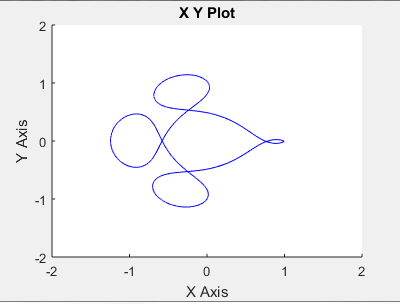
\includegraphics[width = 0.5\textwidth]{step_0025}
   % \caption{1 round with ode5 solver. h = 0.0025. It's ok.}
%\end{figure}



\end{document}